% Mapas exponencial y logarítmico en variedades
% Compilar con: pdflatex exp_log_maps.tex
\documentclass[tikz,border=10pt]{standalone}
\usepackage{tikz}
\usepackage{amsmath}
\usepackage{xcolor}
\definecolor{gdlblue}{RGB}{41, 98, 168}
\definecolor{gdlred}{RGB}{191, 49, 49}
\definecolor{gdlgreen}{RGB}{30, 130, 76}
\definecolor{gdlorange}{RGB}{217, 130, 30}
\definecolor{gdlpurple}{RGB}{118, 56, 138}
\definecolor{gdlgray}{RGB}{140, 140, 140}
\definecolor{gdlyellow}{RGB}{190, 140, 10}
\usetikzlibrary{arrows.meta, decorations.pathmorphing, calc}

\begin{document}
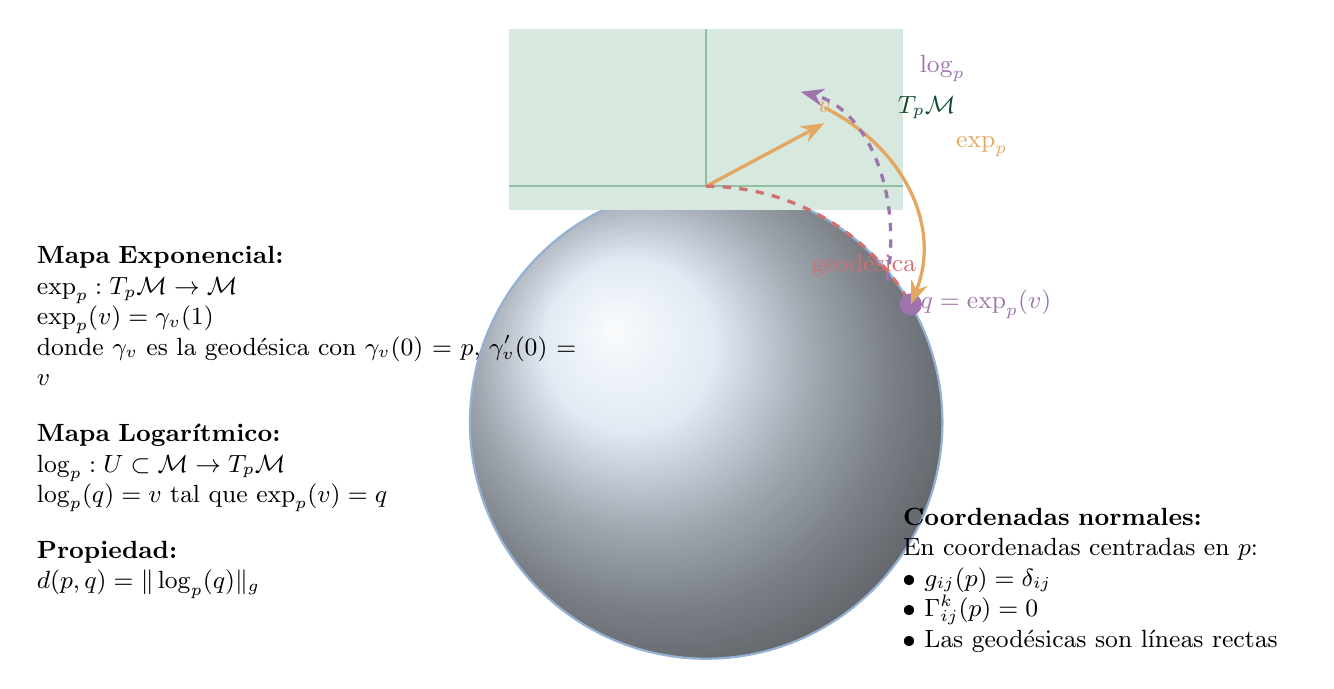
\begin{tikzpicture}[>=Stealth]

% === Variedad (esfera) ===
\shade[ball color=gdlblue!20, opacity=0.9] (0,0) circle (3cm);
\draw[thick, gdlblue!50] (0,0) circle (3cm);

% Punto p
\coordinate (p) at (0, 3);
\fill[gdlred!70] (p) circle (4pt);
\node[above right, font=\small] at (p) {$p$};

% === Espacio tangente en p ===
\begin{scope}[shift={(0, 3)}]
    % Plano tangente
    \fill[gdlgreen!18] (-2.5, -0.3) -- (2.5, -0.3) -- (2.5, 2) -- (-2.5, 2) -- cycle;
    \draw[thick, gdlgreen!50] (-2.5, 0) -- (2.5, 0);
    \draw[thick, gdlgreen!50] (0, 0) -- (0, 2);
    \node[gdlgreen!60!black, font=\small] at (2.8, 1) {$T_p\mathcal{M}$};

    % Vector v en espacio tangente
    \draw[->, very thick, gdlorange!70] (0, 0) -- (1.5, 0.8) node[above, font=\small] {$v$};
\end{scope}

% === Geodésica desde p ===
\draw[very thick, gdlred!70, dashed] (0, 3) arc (90:30:3cm);
\node[gdlred!70, font=\small] at (2, 2) {geodésica};

% Punto q = exp_p(v)
\coordinate (q) at ({3*cos(30)}, {3*sin(30)});
\fill[gdlpurple!70] (q) circle (4pt);
\node[right, font=\small, gdlpurple!70] at (q) {$q = \exp_p(v)$};

% === Flechas de los mapas ===
% exp_p
\draw[->, very thick, gdlorange!70] (1.5, 4) .. controls (2.5, 3.5) and (3, 2.5) .. (q);
\node[gdlorange!70, font=\small] at (3.5, 3.5) {$\exp_p$};

% log_p (inverso)
\draw[->, very thick, gdlpurple!70, dashed] ($(q) + (-0.3, 0.3)$) .. controls (2.5, 3) and (2, 4) .. (1.2, 4.2);
\node[gdlpurple!70, font=\small] at (3, 4.5) {$\log_p$};

% === Propiedades ===
\node[font=\small, text width=7cm] at (-5, 0) {
    \textbf{Mapa Exponencial:}\\
    $\exp_p: T_p\mathcal{M} \to \mathcal{M}$\\
    $\exp_p(v) = \gamma_v(1)$\\
    donde $\gamma_v$ es la geodésica con $\gamma_v(0) = p$, $\gamma_v'(0) = v$\\[1em]
    \textbf{Mapa Logarítmico:}\\
    $\log_p: U \subset \mathcal{M} \to T_p\mathcal{M}$\\
    $\log_p(q) = v$ tal que $\exp_p(v) = q$\\[1em]
    \textbf{Propiedad:}\\
    $d(p, q) = \|\log_p(q)\|_g$
};

% === Coordenadas normales ===
\node[font=\small, text width=5cm] at (5, -2) {
    \textbf{Coordenadas normales:}\\
    En coordenadas centradas en $p$:\\
    • $g_{ij}(p) = \delta_{ij}$\\
    • $\Gamma^k_{ij}(p) = 0$\\
    • Las geodésicas son líneas rectas
};

\end{tikzpicture}
\end{document}
